\section{Assioma dell'infinito e numeri naturali}
Il nostro prossimo obiettivo è definire i numeri naturali. I soli oggetti della teoria degli insiemi sono gl insiemi, per cui va da sé che 
i numeri saranno determinati insiemi. Il nostro scopo non è quindi tanto definire, quanto codificare i numeri naturali per mezzo di insiemi opportuni.
La scelta della codifica non è obbligata: per esempio potremmo decidere che:
\[ \text{``codifica buffa di $n$''} = \underbrace{\{\{\{\ldots \emptyset\ldots\}\}\}}_{\text{$n$ parentesi}}
	\]
Sceglieremo, invece, quest'altra codifica:
\[ n = \{0,1,\ldots,n-1\} = \{x \in \NN | x < n\}
	\]\[ 0 = \emptyset \qquad 1 = \{0\} \qquad 2 = \{0,1\} \qquad 3 = \{0,1,2\} \qquad \text{etc.}
		\]
che presenta alcuni vantaggi: per esempio $n$ è rappresentato da un insieme di $n$ elementi, e dire $m < n$ equivale semplicemente a dire $m \in n$.\\
L'ostacolo è ora parlare di questi oggetti in maniera precisa nel linguaggio della teoria degli insiemi. A dire il vero, potremmo già scrivere una formula $\Phi(n)$ che dice 
``$n$ è un numero naturale'' si tratta di un \textcolor{red}{esercizio} difficile, che sarà reso più facile da idee che vedremo più avanti. Noi non scriviamo questa formula, ma, anche a farlo,
non potremmo comunque dimostrare che esiste un insieme i cui elementi sono i numeri naturali, questo perché gli assiomi visti finora non permettono di uscire dalla classe degli insiemi finiti (degli insiemi ``ereditariamente finiti'',
ad essere precisi: definiremo questi concetto a tempo debito).\\
Servirà un nuovo assioma. E l'idea da sfruttare è che, siccome $n = \{0,\ldots,n-1\}$, per ottenere il successore di $n$, ossia $n+1 = \{0,\ldots,n-1,n\}$ dobbiamo aggiungere a $n$ l'elemento $n$ stesso: $n+1 = n \cup \{n\}$.
Avendo una formula per denotare il successore, possiamo postulare l'esistenza di un insieme chiuso per successori, e questo ci darà $\NN$.

\begin{definition}
	[Successore]
	Definiamo il \vocab{successore} di $x$:
	\[ s(x) \Mydef x \cup \{x\}
		\]
\end{definition}

\begin{definition}
	[Insiemi induttivi]
	Diciamo che $A$ è un \vocab{insieme induttivo} se contiene $\emptyset$ ed è chiuso per successori \footnote{Ciò non esclude che ci possano essere altri elementi oltre a $\emptyset$ che non siano successori (questa cosa è sempre falsa in $\omega$).}, ossia:
	\[ \text{$A$ è induttivo} \iff \emptyset \in A \land \forall x \in A \; s(x) \in A
		\]
\end{definition}

\begin{axiom}
	[Assioma dell'infinito]
	\label{ax7}
	Esiste un insieme induttivo.
	\[ \exists A (\emptyset \in A \land (\forall x \in A \; s(x) \in A))
		\]
\end{axiom}

Finalmente definiamo l'insieme dei numeri naturali - che, per qualche buffa ragione, chiamiamo $\omega$ - come l'intersezione della classe, non vuota per l'assioma dell'infinito,
di tutti gli insiemi induttivi.\footnote{Aver introdotto l'assioma dell'infinito
ci assicura che tale intersezione è non vuota, e ciò basta affinché $\omega$ sia un insieme (in caso contrario avremmo avuto l'intersezione del vuoto, che, come visto, non è un insieme).}

\begin{definition}[Numeri naturali]
	L'insieme $\omega$ è l'intersezione di tutti gli insiemi induttivi, ossia $\omega$ è l'unico insieme tale che:
	\[ \forall x (x \in \omega \leftrightarrow(\forall A \; \text{``$A$ è induttivo''}\rightarrow x \in A)) \footnote{Cioè $x$ è in $\omega$ se e solo se è elemento
	di qualsiasi insieme induttivo (nella \underline{classe} degli insiemi induttivi), e, inoltre, essendo l'intersezione di una classe, è in particolare un insieme (perché per definizione
	stiamo intersecando gli elementi di una classe, che sono insiemi).}
		\]
\end{definition}

Adesso che abbiamo $\omega$, possiamo facilmente dimostrare che ogni dato numero naturale vi appartiene.

\begin{definition}[Codifica dei numeri naturali]
	Definiamo:
	\[ 0 \Mydef \emptyset \qquad 1 \Mydef s(0) \qquad 2 \Mydef s(1) \qquad 3 \Mydef s(2) \qquad \text{etc.}
		\]
\end{definition}

\begin{exercise}
	Dimostra che $0,1,2,3 \in \omega$.
\end{exercise}

\begin{soln}
	Avendo definito $\omega$ come:
	\[ \omega = \bigcap_{\text{$A$ induttivo}} A
		\]
	sappiamo che $\emptyset \in A$, per ogni insieme induttivo (per definizione), dunque $0 \in \omega$. Inoltre vale che l'intersezione di insiemi induttivi è chiusa per successore (e quindi per quanto appena mostrato è a sua volta un insieme induttivo), infatti:
	\[ \forall x \in \bigcap_{\text{$A$ induttivo}} A \leftrightarrow \forall A \, \text{$A$ induttivo}\, (x \in A)
		\]
	ed essendo tutti gli $A$ chiusi per successore (in quanto induttivi) segue che:
	\[ s(x) \in \bigcap_{\text{$A$ induttivo}} A \implies s(x) \in \omega
		\]
	Pertanto, avendo osservato che $0 \in \omega$, si avrà anche che $1 = s(0) \in \omega$, $2 = s(1) \in \omega$, $3 = s(2) \in \omega$ e così via.
\end{soln}

Un esercizio un po' più difficile è esibire insiemi che non appartengono a $\omega$.

\begin{exercise}
	Dimostra che $\{\{\emptyset\}\} \not \in \omega$.\footnote{\textbf{\underline{Idea}}: Esibisci un insieme induttivo che non contiene $\{\{\emptyset\}\}$.}
\end{exercise}

\begin{soln}
	Osserviamo che $\{\{\emptyset\}\}$ non è un successore, se fosse che $s(x) = x \cup \{x\} = \{\{\emptyset\}\}$, dato che $x$ è elemento di $s(x)$ e che $\{\{\emptyset\}\}$ ha un solo elemento, per \hyperref[ax2]{estensionalità} deve essere che che $x = \{x\} = \{\emptyset\}$ (ossia tutti gli elementi di $s(x)$ devono essere 
	uguali all'unico elemento di $\{\{\emptyset\}\}$). Pertanto avremmo che $x = \{\emptyset\}$, ma $s(x) = s(\{\emptyset\}) = \{\emptyset\} \cup \{\{\emptyset\}\} =\footnote{Volendo essere pignoli possiamo usare la definizione dell'unione come il prendere gli elementi degli elementi: $\{\emptyset\} \cup \{\{\emptyset\}\} = \bigcup \{\{\emptyset\},\{\{\emptyset\}\}\}$,
	e l'unione di tale insieme è formata appunto da tutti gli elementi degli elementi (quindi naturalmente il vuoto $\emptyset$ e anche $\{\emptyset\}$).} \{\emptyset,\{\emptyset\}\}$, ma $\{\emptyset\} \ne \emptyset$, perché $\{\emptyset\}$ è non vuoto e $\emptyset$ è proprio il vuoto.\\
	Avendo dimostrato che $\{\{\emptyset\}\}$ non è né un successore né (ovviamente) il vuoto, ci basta mostrare mostrare che non appartiene ad un insieme induttivo $A$ che non ha altri elementi (oltre a $\emptyset$) che non sono successori. Dando per buono che $\omega$ non contenga elementi che non sono successori, si ottiene che
	$\{\{\emptyset\}\} \not \in \omega$.\footnote{Non abbiamo usato l'hint di Mamino e abbiamo usato un fatto non dimostrato.}
\end{soln}

\subsection{Gli assiomi di Peano}
Per convincerci, però, che $\omega$ è, a buon diritto, l'insieme dei numeri naturali, serve qualcosa di più. Classicamente, i numeri naturali si definiscono per mezzo degli
\vocab{assiomi di \href{https://it.wikipedia.org/wiki/Giuseppe_Peano}{\textcolor{purple}{Peano}}}. Questi assiomi, che caratterizzano a meno di isomorfismi l'insieme $\NN$ dotato della funzione di successore, \textbf{per noi diventano dei teoremi} che
dimostreremo a proposito dell'insieme $\omega$\footnote{Cioè gli assiomi di Peano diventano enunciati dimostrabili all'interno della ZFC.}. In questo senso\footnote{Classicamente gli assiomi definivano $\NN$ a meno di isomorfismo, mostrando che $\omega$ li soddisfa siamo sicuri di avere l'oggetto (insieme) $\NN$ definito da tali assiomi nella ZFC, e tale oggetto è appunto $\omega$.}, quindi, $\omega$ codifica legittimamente i numeri naturali.

\begin{definition}
	[Assiomi di Peano al secondo ordine\protect\footnote{qualunque cosa questo significhi...}]
	Dato un insieme $\NN$, un elemento $0 \in \NN$, e una funzione:
	\[ \text{succ} : \NN \to \NN
		\]
	diciamo che $(\NN,0,\text{succ})$\footnote{La 3-upla ordinata formata dai tre insiemi $\NN$,$0$,succ: (($\NN$,0),succ)$= \{(\NN,0),\{(\NN,0),\text{succ}\}\} = \{\{\NN,\{\NN,0\}\},\{\{\NN,\{\NN,0\}\},\text{succ}\}\}$.} soddisfa gli assiomi di Peano se:
	\begin{enumerate}[(a)]
		\item \label{a}Il successore è iniettivo:
		\[ \forall n,m \in \NN \; \text{succ}(m) = \text{succ}(n) \rightarrow m = n \, \footnote{L'altra freccia è banale e sarà data sempre per scontata.}
			\]
		\item \label{b}Lo zero non è un successore:
		\[ \not\exists n \in \NN \; \text{succ}(n) = 0
			\]
		\item \vocab{Principio di induzione}: data una qualunque formula insiemistica (proprietà) $\Phi(n)$ vale:
		\[ (\Phi(0) \land \forall n \in \NN \; \Phi(n) \rightarrow \Phi(\text{succ}(n))) \rightarrow \forall n \in \NN \; \Phi(n)
			\]
	\end{enumerate}
\end{definition}


\begin{figure*}[h]
		\centering
		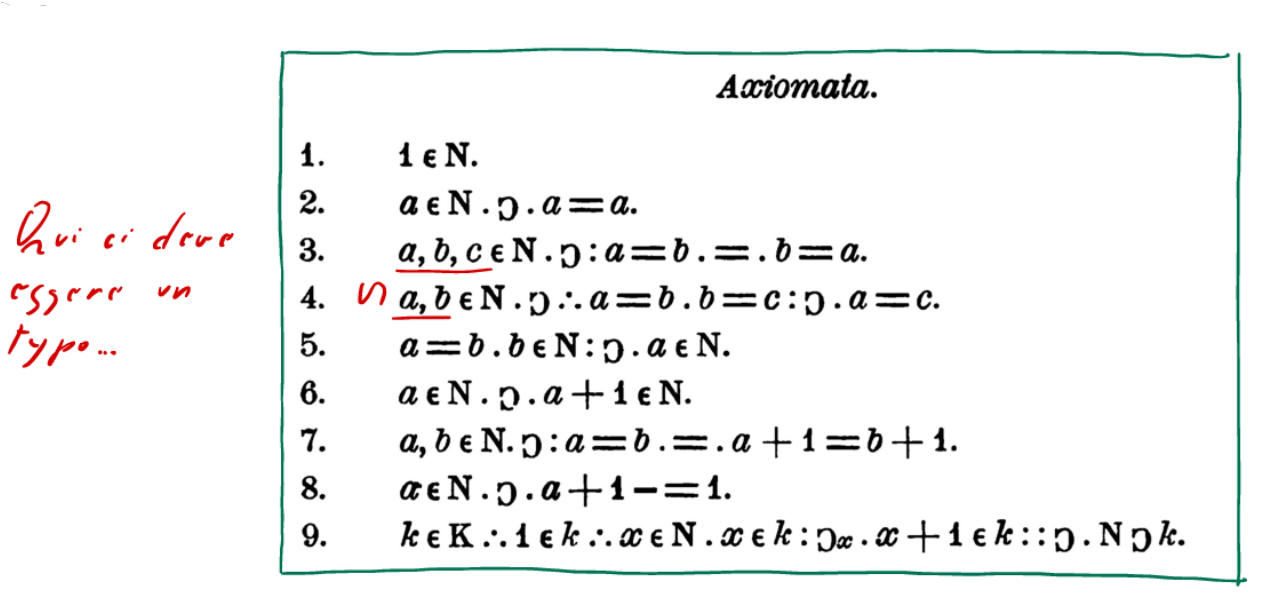
\includegraphics[width=10.5cm]{immagini/peano.png}
		\captionsetup{labelformat=empty}
		\caption{Apparivano così in ``\emph{Arithmetices principia}'', nel 1889, gli assiomi di Peano.}
\end{figure*}


\begin{theorem}[$\omega$ soddisfa gli assiomi di Peano]
	La funzione $\text{succ}: \omega \rightarrow \omega : n \mapsto s(n)$, è ben definita e $(\omega,\emptyset,\text{succ})$
	soddisfa gli assiomi di Peano.
\end{theorem}

\begin{proof}
	Prima di procedere con le verifiche controlliamo che la funzione $\text{succ} = s$ sia ben definita.
	Occorre assicurarsi che se $n \in \omega$, allora $\text{succ}(n) = s(n) \in \omega$. Fissiamo $n \in \omega$
	e consideriamo un qualunque insieme induttivo $A$. Siccome $A$ è induttivo $\omega \subseteq A$, quindi $n \in A$, e, di conseguenza $s(n) \in A$. Per 
	l'arbitrarietà di $A$, allora, $s(n)$ appartiene a ogni insieme induttivo (quindi all'intersezione, ovvero $\omega$).\\
	Dimostriamo ora che $\omega$ rispetta gli assiomi di Peano. Iniziamo con dimostrare (b) e (c), poi passeremo ad (a):
	\begin{enumerate}
		\item[(b)] Supponiamo, per assurdo, $s(n) = \emptyset$. Abbiamo allora che:
		\[ n \in s(n) =  n \cup \{n\} = s(n) = \emptyset
			\]
		contro la definizione di $\emptyset$.
		\item[(c)] Per verificare il principio di induzione, date le ipotesi, occorre verificare che il sottoinsieme di $\omega$ degli elementi per cui è vera $\Phi(n)$ è proprio tutto $\omega$, dunque 
		se dimostriamo che l'insieme $A = \{n \in \omega | \Phi(n)\} \subseteq \omega$ è induttivo, avendo gratis il primo contenimento, si ha $\omega = A$.
		\begin{enumerate}[(1)]
			\item Per ipotesi abbiamo che $\Phi(\emptyset)$, quindi $\emptyset \in A$.
			\item $n \in A \overset{\text{def. $A$}}{\implies} \Phi(n) \overset{\text{passo indutt.}}{\implies} \Phi(\text{succ}(n)) = \Phi(s(n)) \overset{\text{def. $A$}}{\implies} s(n) \in A$
		\end{enumerate}
		\item[(a)] La dimostrazione passa attraverso due lemmi.
					\begin{lemma}
					[Lemma 1]
					L'unione di un elemento di $\omega$ è contenuta nell'elemento: $\forall n \in \omega \; \bigcup n \subseteq n$.\footnote{E.g. $\bigcup 3 = \bigcup \{0,1,2\} = \{0,1\} = 2$.}
					\end{lemma}
					\begin{proof}
						Avendo dimostrato in (c) che in $\omega$ vale l'induzione possiamo usarla con $\Phi(n) \Mydef \bigcup n \subseteq n$. 
						\[
							\begin{split}
							\boxed{\Phi(\emptyset)} & \qquad \bigcup \emptyset = \emptyset \subseteq \emptyset \\
							\boxed{\Phi(n) \rightarrow \Phi(s(n))} & \qquad \bigcup s(n) = \bigcup(n \cup \{n\}) \overset{\star}{=} \underbrace{\left(\bigcup n\right)}_{\subseteq n} \cup n \overset{\text{Hp. indutt.}}{\subseteq} n \cup n = n \subseteq s(n)
							\end{split}
						\]
						(si noti che il passo base è coerente con le definizioni delle abbreviazioni date), e $\star$ vale in quanto:
						\[ \begin{split}
							x \in \bigcup(n \cup \{n\}) \overset{\text{def.}}{\iff} &\quad \exists y ( x \in y) \land (y \in (n \cup\{n\})) \\
														\overset{\text{caratt. $\cup$}}{\iff} &\quad \exists y( x \in y) \land (y \in n \lor y = n)\\
														\overset{\text{distrib. $\land$}}{\iff} &\quad \exists y \; ( x \in y \land y \in n) \lor (x \in y \land y = n)\\
														\iff &\quad \exists y ( x \in y \land y \in n) \lor \exists y(x \in y \land y = n)\\
														\overset{\text{def.}}{\iff} &\quad x \in \bigcup n \lor x \in n\\
														\overset{\text{caratt. $\cup$}}{\iff} &\quad x \in \left(\bigcup n\right) \cup n
						\end{split}
							\]
						(dove alla secondo membro della seconda equivalenza abbiamo che $y \in \{n\}$ e per \hyperref[ax2]{estensionalità} equivale a $y = n$.).
					\end{proof}
					\begin{lemma}
						[Lemma 2]
						L'unione dei successori di un elemento in $\omega$ è proprio l'elemento: $\forall n \in \omega \; \bigcup s(n) = n$.
					\end{lemma}
					\begin{proof}
						Ricopiando quanto fatto nel passo induttivo della dimostrazione precedente abbiamo:
						\[ \bigcup s(n) = \bigcup (n \cup \{n\}) = \left(\bigcup n\right) \cup n \overset{\star}{\subseteq} n
							\]
						dove in $\star$ abbiamo usato che $\bigcup n \subseteq n$, non per ipotesi induttiva (visto che non stiamo facendo alcuna induzione), ma stiamo usando direttamente il risultato del Lemma 1.
						Naturalmente vale anche che $n \subseteq \bigcup s(n)$ (ogni elemento di $n$ è elemento dell'elemento $n$ in $s(n)$), dunque vale la tesi.
					\end{proof}
					Finalmente abbiamo che, per il Lemma 2:
					\[ s(m) = s(n) \implies \bigcup s(m) = \bigcup s(n) \overset{\text{Lemma 2}}{\iff} m = n
						\]
					dove la prima freccia è data dal fatto che stiamo considerando l'unione di insiemi uguali, dunque succ$: \omega \rightarrow \omega$ è iniettiva.
	\end{enumerate}
\end{proof}

\subsection{L'ordine di omega}
Conviene, adesso, sviluppare un po' di tecnologia per manipolare i numeri interi. Dopo, dimostreremo altresì che gli assiomi di Peano hanno un unico modello $(\NN, 0, \text{succ})$
a meno di isomorfismi.

\begin{notation}[Relazione di ordine su $\omega$]
	Dati $m,n \in \omega$, scriviamo:
	\[ m < n \Mydef m \in n \footnote{Per essere precisi non stiamo usando $\in$ come una relazione (visto che abbiamo assunto all'inizio che fosse un simbolo del linguaggio della teoria degli insiemi),
	ma stiamo definendo $< \Mydef \{(m,n) \in \omega \times \omega | m \in n\}$. Inoltre se aggiungiamo la diagonale $\Delta_\omega$ a $<$, otteniamo $\leq$ (cioè $m \leq n \Mydef (m \in n) \lor (m = n)$), che, come visto, è legata alla corrispondente relazione d'ordine 
	stretto, e godrà di tutte le stesse proprietà (come vedremo man mano).}
		\]
\end{notation}

\begin{proposition}[Ordinamento totale di $\omega$]
	La relazione $<$ è un ordine totale su $\omega$. 
\end{proposition}

Per dimostrare questa proposizione, sono comodi alcuni lemmi.

\pagebreak

\begin{remark}[Successore del secondo termine in un'appartenenza]
	\label{succ2}
	Si osserva che valgono le seguenti cose:
	\begin{enumerate}[(1)]
		\item $m \in n \rightarrow m \in s(n)$, infatti $n \subseteq n \cup \{n\} = s(n)$ (banalmente se $m$ è contenuto in $n$ allora è contenuto anche nel suo successore).
		\item $m \in s(n) \rightarrow (m \in n \lor m = n)$, ciò se $m$ è nel successore di $n$, allora è $n$ stesso o un suo elemento, infatti:
		 \[ \begin{split}
			m \in s(n) = n \cup \{n\} & \iff m \in (n \cup \{n\}) \\
									& \iff (m \in n) \lor (m \in \{n\}) \\
									&\iff (m \in n) \lor (m = n)
		 \end{split}
			\]
		(nella seconda equivalenza si è usata la caratterizzazione data dell'appartenenza ad un unione di insiemi, e nella terza il fatto che se $m$ appartiene ad un singoletto, allora per \hyperref[ax2]{estensionalità} è proprio l'unico elemento del singoletto).
	\end{enumerate}
\end{remark}

\begin{lemma}[Successore del primo termine in un'appartenenza]
	$\forall a,b \in \omega \; a \in b \rightarrow (s(a) \in b \lor s(a) = b)$.\footnote{Moralmente: se un numero è strettamente più piccolo di un altro, o il suo successore è a sua volta più piccolo del secondo numero, o coincide con quest'ultimo.}
\end{lemma}

\begin{proof}
	Procediamo per induzione su $b$.
	\begin{itemize}
		\item[$\boxed{\text{caso $b = 0$}}$] $a \in \emptyset \rightarrow \ldots$ vera a vuoto, perché $a \in \emptyset$ è falsa (dunque l'implicazione è sempre vera, indipendentemente dal valore di verità dell'antecedente).
		\item[$\boxed{\text{caso $b = s(n)$}}$] L'ipotesi induttiva è $a \in n \rightarrow (s(a) \in n \lor s(a) = n)$. Dobbiamo dimostrare:
		\[ a \in s(n) \rightarrow (s(a) \in s(n) \lor s(a) = s(n))
			\]
		abbiamo che $a \in s(n) \iff a \in n \cup \{n\} \iff a \in n \lor a = n$. Quindi abbiamo due casi:
		\[ \begin{split}
			& a \in n \overset{\text{Hp. indutt.}}{\implies} (s(a) \in n) \lor (s(a) = n) \overset{\text{def. $s(n)$}}{\iff} s(a) \in s(n) \\
			& a = n \iff s(a) = s(n)
		\end{split}
			\]
		(la seconda equivalenza è giustificata dal fatto che abbiamo dimostrato che la funzione successore in $\omega$ è iniettiva).
	\end{itemize}
\end{proof}

Possiamo ora dimostrare la proposizione iniziale.

\begin{proof}
	Per verificare che $<$ è una relazione di ordine stretto totale, dobbiamo verificare che è irriflessiva, transitiva e totale (cioè presi qualsiasi due elementi di $\omega$ la loro coppia ordinata appartiene a $<$).
	\begin{itemize}
		\item[$\boxed{\text{transitività}}$] Vogliamo verificare che $(a \in b \land b \in c) \rightarrow a \in c$. Procediamo per induzione su $c$:
		\begin{itemize}
			\item[$\boxed{\text{caso $c = 0$}}$] la premessa $b \in c$ è falsa, quindi l'implicazione è vera a vuoto (l'antecedente è sempre falso, quindi l'implicazione sempre vera).
			\item[$\boxed{\text{caso $c = s(n)$}}$] assumiamo per ipotesi induttiva $(a \in b \land b \in n) \rightarrow a \in n$, e vogliamo dimostrare:
				\[ (a \in b \land b \in s(n)) \rightarrow a \in s(n)
					\]
				Osserviamo che $a \in b \implies a \in s(b)$, e che $b \in s(n) \overset{\text{Lemma}}{\implies} s(b) \in s(n) \lor s(b) = s(n)$, abbiamo quindi due casi in base a $s(b)$:
				\[ \begin{split}
					& s(b) = s(n) \implies a \in s(b) = s(n) \implies a \in s(n)\\
					& s(b) \in s(n) \implies a \in s(b) \in s(n) \implies a \in s(n)
				\end{split}
					\]
				questo usando il lemma precedente, potevamo anche scegliere di usare l'osservazione per dire che $b \in s(n) \implies b = n \lor b \in n$ e ottenere ancora i casi:
				\[  \begin{split}
					& b = n \implies a \in b = n \overset{\text{Oss.}}{\implies} a \in s(n) \\
					& b \in n \implies a \in b \in n \implies a \in n \overset{\text{Oss.}}{\implies} a \in s(n)
					\end{split}
					\]
		\end{itemize}
		\item[$\boxed{\text{irriflessività}}$] Vogliamo verificare $\neg \,a \in a$, e lo facciamo per induzione su $a$:
		\begin{itemize}
			\item[$\boxed{\text{caso $a = 0$}}$] $\neg \, \emptyset \in \emptyset$, vero per definizione di $\emptyset$.
			\item[$\boxed{\text{caso $a = s(n)$}}$] L'ipotesi induttiva è $\neg \, n \in n$, e vogliamo verificare che $\neg s(n) \in s(n)$. Procediamo per assurdo, supponiamo che $s(n) \in s(n)$, e per l'osservazione abbiamo due casi:
			\[ \begin{split}
				& s(n) = n \implies n \in n \; \lightning\\
				& s(n) \in n \implies n \in s(n) \in n \implies n \in n \; \lightning
			\end{split}
				\]
			($n \in n$ è falso perché per ipotesi induttiva $\neg(n \in n)$ è vero).
		\end{itemize}
		\item[$\boxed{\text{totalità}}$] Vogliamo dimostrare che $\forall a,b \in \omega (a \in b) \lor (a = b) \lor (b \in a)$. Iniziamo per induzione su $a$:
		\begin{itemize}
			\item[$\boxed{\text{caso $a = 0$}}$] La tesi diventa $\forall b \in \omega (\emptyset \in b) \lor (\emptyset = b) \lor (b \in \emptyset) \footnote{Ovviamente quest'ultimo caso è sempre faslo e quindi può essere escluso.}$. Procediamo quindi per induzione su $b$:
			\begin{itemize}
				\item \textbf{\underline{caso $b = 0$}} La tesi diventa $(\emptyset \in \emptyset) \lor (\emptyset = \emptyset)$, dove naturalmente la prima affermazione è sempre falsa, mentre la seconda è sempre vera, dunque la tesi è vera.
				\item \textbf{\underline{caso $b = s(m)$}} La tesi è $(\emptyset \in s(m)) \lor (\emptyset = s(m))$, con ipotesi induttiva $(\emptyset \in m) \lor (\emptyset = m)$. Abbiamo quindi due casi in base all'ipotesi induttiva:
				\[ \begin{split}
					& \emptyset \in m \implies \emptyset \in s(m) \\
					& \emptyset = m \implies \emptyset \in \{\emptyset\} = s(m)
				\end{split}
					\]
				in entrambi casi è vera la tesi perché è sempre vero il primo termine.
			\end{itemize}
			\item[$\boxed{\text{caso $a = s(n)$}}$] La tesi è $\forall b \in \omega (s(n) \in b) \lor (s(n) = b) \lor (b \in s(n))$, mentre l'ipotesi induttiva è $(n \in b) \lor (n = b) \lor (b \in n)$. Dall'ipotesi induttiva abbiamo quindi tre casi:
				\[ \begin{split}
					& n \in b \overset{\text{Lemma}}{\implies} s(n) \in b \lor s(n) = b \\
					& n = b \overset{\text{Iniett. del succ.}}{\implies} s(n) = s(b) \implies b \in s(b) = s(n) \implies b \in s(n)\\
					& b \in n \overset{\text{Oss.}}{\implies} b \in s(n) \implies b \in a 
				\end{split}
					\]
				in tutti e tre i casi almeno una delle tre proposizioni della tesi è vera, dunque la tesi è sempre vera.
		\end{itemize}
	\end{itemize}
\end{proof}

\begin{remark}[$\leq$ ordina totalmente $\omega$]
	Avendo dimostrato che $<$ è un ordine totale su $\omega$, abbiamo dimostrato in automatico che anche $\leq = < \cup \Delta$ lo è, infatti, per la corrispondenza tra i due (come si è visto precedentemente in una proposizione), anche le definizioni di ordine totale sono corrispondenti (in particolare per 
	$\leq$ ci basta che valga una tra $\leq$ e $\geq$, se valgono entrambe c'è l'=, mentre per $<$ chiedevamo nella definizione che valesse $<$, $>$ o $=$, quindi se nella dimostrazione precedente avessimo usato $\leq$ al posto di $<$ avremmo ottenuto lo stesso risultato perché le richieste nella definizione di ordine totale sono le stesse).
\end{remark}

\begin{corollary}[Rappresentazione dei numeri naturali]
	Un numero naturale è l'insieme dei numeri naturali minori di lui.
	\[ \forall m \in \omega \; m = \{n \in \omega | n < m\}
		\]
\end{corollary}

\begin{proof}
	Vogliamo dire che $m = \{ n \in \omega | n \in m\}$, ossia per definizione di sottoinsieme che $m \subseteq \omega$. Per induzione: $\emptyset \subseteq \omega$ è vera (perché $\omega$ è induttivo).
	Assumiamo che $m \subseteq \omega$, allora $s(m) = \underbrace{m}_{\subseteq \omega} \cup \{m\}$ e $\{m\} \subseteq \omega$ perché $m \in \omega$ per ipotesi iniziale, quindi si conclude che $s(m) \subseteq \omega$.
\end{proof}

\begin{corollary}[Più piccolo = contenuto]
	$\forall m,n \in \omega (m \leq n \leftrightarrow m \subseteq n$).\footnote{Naturalmente il lemma vale anche con $<$ e $\subsetneq$.}
\end{corollary}

\begin{proof}
	Siccome $\omega$ è totalmente ordinato, si danno due casi (nel primo dimostro $\rightarrow$, nel secondo dimostro che la negazione della premessa implica la negazione della conseguenza, che è equivalente [via contronominale] a $\leftarrow$):
	\begin{align*}
		& m \leq n \implies \forall x \in \omega (x < m \rightarrow x < n) \overset{\text{def. $<$}}{\implies} \forall x \in \omega (x \in m \rightarrow x \in n) \overset{\text{def. $\subseteq$}}{\implies} m \subseteq n \\
	    & n < m \implies n \in m \; \text{tuttavia} \; n \not\in n \; \text{quindi non può essere che $m \subseteq n$ ovvero} \; m \not\subseteq n
	\end{align*}
	($n \not \in n$ perché abbiamo dimostrato che $<$ è di ordine stretto su $\omega$, quindi irriflessiva, inoltre, nella dimostrazione del primo caso, si osserva che nel secondo passaggio è
	indifferente usare $<$ o $\leq$ nell'enunciato e dimostrazione del corollario\footnote{Mamino li mischia, ma valgono entrambi gli enunciati e le dimostrazioni.}.
\end{proof}
\pagebreak
\subsection{Induzione forte e principio del minimo}
\begin{theorem}
	[Principio di induzione - forma forte]
	Data una formula insiemistica $\Phi(x)$, vale:
	\[ (\forall n \in \omega (\forall x < n \; \Phi (x)) \rightarrow \Phi(n)) \rightarrow \forall n \in \omega \; \Phi(n)
		\]
	ovvero, se assumendo $\Phi(x)$ per tutti gli $x < n$, abbiamo $\Phi(n)$, allora $\Phi(n)$ è vera per tutti i numeri $n$.
\end{theorem}

\begin{remark}
	Chiaramente questa forma è ``forte'' perché permette di assumere un'ipotesi induttiva più forte dell'induzione di Peano. In quella, infatti, si deve dedurre $\Phi(n)$ a 
	partire da $\Phi$ del numero precedente. Qui, invece, possiamo far conto di sapere $\Phi$, non solo per il precedente, ma per tutti i numeri minori di $n$.
\end{remark}

\begin{proof}
	Definiamo $\psi(m) \Mydef \forall x < m \; \Phi(x)$ e dimostriamo per induzione debole che $\forall m \in \omega \; \psi(m)$, \textcolor{MidnightBlue}{ cioè che per ogni fissato naturale $\Phi$ è vera per i naturali più piccoli},
	in tal modo, per ogni $n \in \omega$ sappiamo che è vera $\psi(n+1) \implies \Phi(n)$, che è proprio la tesi.
	\begin{itemize}
		\item[$\boxed{m = 0}$] Abbiamo che $\psi(0) = \forall x < 0 \; \Phi(x) \equiv \forall x (x < 0 \to \Phi(x))$, che è vera a vuoto in quanto $x < 0 \equiv x \in \emptyset$ che è sempre falso, dunque l'implicazione tra partentesi è sempre vera.
		\item[$\boxed{m \implies m + 1}$] Assumiamo che $\psi(m) = \forall x < m \; \Phi(x)$ sia vera e mostriamo che $\psi(m) = \forall x < m + 1 \; \Phi(x)$ è vera. Per un lemma visto $x < s(m) \implies x < m \lor x = m$, nel primo caso $\Phi(x)$ è vera per ipotesi induttiva.
		Nel caso di $\Phi(m)$, abbiamo per ipotesi che \textcolor{purple}{$\forall n \in \omega (\forall x < n \; \Phi (x)) \rightarrow \Phi(n)$}, dunque, per $n = m$, abbiamo visto nel primo caso che $\forall x < m \; \Phi(m)$, per cui l'ipotesi (vera) ha antecedente vero, che ci dà necessariamente conseguente $\Phi(m)$ vero.
	\end{itemize}
\end{proof}

\begin{theorem}
	[Principio del minimo]
	Sia $A \subseteq \omega$. Se $A \ne \emptyset$ allora esiste $n \in A$ tale che $\forall x \in A \; n \leq x$. Ovvero, ogni sottoinsieme non vuoto di $\omega$ ha un minimo elemento.
\end{theorem}

\textcolor{MidnightBlue}{\underline{Possibile idea di dimostrazione}: dimostriamo per induzione forte che se $n \in A$ - che è equivalente a $A\subseteq \omega \land A \ne \emptyset$ -, allora $A$ ha un minimo. Per ipotesi induttiva assumiamo che $\forall x < n \; x \in A \to A$ ha minimo, e dimostriamo che se $n \in A$, allora 
$A$ ha minimo. Dato $n \in A$, se esiste $x \in n$ tale che $x \in A$, allora $A$ ha minimo per ipotesi induttiva, altrimenti, se $\forall x < n \; x \not \in A$, allora $n$ è il minimo di $A$.}

\begin{proof}
	Dimostriamo la contronominale della tesi, ovvero se $A \subseteq \omega$ non ha un elemento minimo, allora $A$ è vuoto, cioè $\forall n \in \omega \; n \not \in A$. Procediamo per induzione forte, assumendo per ipotesi induttiva che $\forall x < n \; x \not \in A$, mostriamo che $n \not \in A$.
	Più precisamente vogliamo dimostrare che $(\forall x < n \; x \not \in A) \to n \not \in A$, ma ciò è equivalente al fatto che $A$ non abbia un minimo:
	\begin{align*}
		(\forall x < n \; x \not \in A) \to n \not \in A &\iff \neg(\exists x < n \; x \in A) \to n \not \in A \\
														 &\iff n \in A \to \exists x < n \; x \in A &&\text{(contronominale)}\\
														 &\iff \text{$A$ non ha minimo}
	\end{align*}
	abbiamo quindi dimostrato che l'implicazione che vogliamo dimostrare è equivalente all'ipotesi per cui è vera, inoltre per l'ipotesi induttiva l'antecedente dell'implicazione è vero, per cui, dalla tavola di verità,
	l'unica possibilità è che anche il conseguente $n \not \in A$ sia vero. Ciò verifica il passo induttivo e quindi l'induzione forte ci garantisce la contronominale della tesi - che naturalmente è equivalente a quest'ultima -.
\end{proof}

\begin{remark}
	Per completare l'equivalenza tra induzione, induzione forte e principio del minimo, andrebbe dimostrato anche che principio del minimo$\implies$induzione.
\end{remark}

\begin{definition}[Insieme ben ordinato]
	Un insieme totalmente ordinato $(S, <)$ si dice \vocab{bene ordinato} se ogni sottoinsieme non vuoto ha un minimo.\footnote{Cioè se vale il principio del minimo c(come vale in $\omega$).}
	\[ \forall A \subseteq S \; A \ne \emptyset \rightarrow \exists m \in A \; \forall x \in A \; m \leq x
		\]
\end{definition}

La nozione di buon ordine è stata introdotta da Cantor agli albori della teoria degli insiemi, e giocherà un ruolo centrale in questo corso.

\begin{example}
	$(\omega, <)$ è un insieme bene ordinato\footnote{Si usa la notazione di coppia ordinata per indicare sia l'insieme sia la relazione che c'è sopra.} per quanto visto nel teorema precedente.
\end{example}

\begin{exercise}
	Dimostra che $X = s(s(s(\omega)))$ è bene ordinato dalla relazione $a < b \Mydef a \in b$.
\end{exercise}

\begin{soln}
	Dato $(\omega,<)$, basta considerare la seguente relazione:
	\[ \prec := < \cup (\omega \times \{\omega\}) \cup (s(\omega) \times \{s(\omega)\}) \cup (s(s(\omega)) \times \{s(s(\omega))\})\,\footnote{Che formalmente è un sottoinsieme di $s(s(s(\omega))) \times s(s(s(\omega)))$.}
		\]
	dove $(x,y) \in \prec \leftrightarrow x \in y$. Si vede quindi che $(s(s(s(\omega))),\prec)$ è un ordine totale (fondamentalmente perché $<$ lo è, 
	e le coppie che abbiamo aggiunto sono costruite apposta per rispettare la definizione di ordine [stretto] totale). Abbiamo costruito $\prec$ in modo che 
	$\forall n \in \omega \; n \prec \omega$, inoltre vale anche [per costruzione] che $\omega \prec s(\omega) \prec s(s(\omega))$, dunque, dato $S \subseteq s(s(s(\omega)))$,
	se $S \cap \omega \ne \emptyset$, allora il minimo esiste ed è dato da $\min_<(S \cap \omega)$. Se $S \cap \omega = \emptyset$ (ovvero se $S$ è un sottoinsieme di $\{\omega,s(\omega),s(s(\omega))\}$),
	allora per definizione di $\prec$ (come scritto sopra), per tutti i sottoinsiemi possibili abbiamo sempre un minimo [per la totalità di $\prec$]. Pertanto $\forall S \subseteq s(s(s(\omega)))$ c'è un minimo
	e quindi in $s(s(s(\omega)))$ vale il principio del minimo, cioè è ben ordinato.
\end{soln}

\subsection{Ricorsione numerabile}
La ricorsione è il procedimento per cui si costruisce una funzione $f : \omega \rightarrow \text{qualcosa}$, definendo $f(s(n))$ a partire da $f(n)$, o,
più in generale da $f(\emptyset),\ldots,f(n)$. Questo è un procedimento fondamentale: potremmo dire che è IL modo di pensare gli infidi puntini ($\ldots$). Vediamo qualche esempio.

\begin{example}
	[Operazioni aritmetiche]
	Possiamo definire somma e prodotto come:
	\[ \begin{cases}
		a + \textcolor{red}{0} = a \\
		a + \textcolor{red}{s(b)} = s(a + b)
	\end{cases}
	\qquad
	\begin{cases}
		a \cdot \textcolor{red}{0} = 0\\
		a \cdot \textcolor{red}{s(b)} = a \cdot b + a
	\end{cases}
		\]
	anziché $a + b = \underbrace{s(s(\ldots a \ldots))}_{\text{$b$ successori}}$ (abbiamo il caso base con 0, e poi si procede ricorsivamente dal caso base fino a $b$) e $a \cdot b = \underbrace{a + a + \ldots + a}_{\text{$b$ volte}}$ (ricorsivamente ad un certo 
	punto si partirà da $a$ e si inizierà a sommare).
\end{example}

\begin{example}
	[Potenza e fattoriale]
	Possiamo definire ricorsivamente potenze e fattoriali come segue:
	\[ \begin{cases}
		a^{\textcolor{red}{0}} = 1\\
		a^{\textcolor{red}{s(b)}} = a^b \cdot a
	\end{cases}
	\qquad
	\begin{cases}
		\textcolor{red}{0}! = 1\\
		\textcolor{red}{s(a)}! = a! \cdot s(a)
	\end{cases}
		\]
	anziché $a^b = \underbrace{a \cdot a \cdot \ldots \cdot a}_{\text{$b$ volte}}$ e $a! = 1 \cdot 2 \cdot \ldots \cdot (a - 1) \cdot a$.
\end{example}

\begin{example}
	[Sommatoria]
	Possiamo definire la sommatoria come:
	\[\begin{cases}
		\displaystyle
		\sum_{i = 0}^{\textcolor{red}{0}} f(i) = 0\\
		\displaystyle
		\sum_{i = 0}^{\textcolor{red}{s(a)}} f(i) = \left(\sum_{i=0}^{a} f(i) \right) + f(s(a))
	\end{cases}
		\]
	anziché $\displaystyle\sum_{i = 0}^a f(i) = f(0) + f(1) + \ldots + f(a)$ (cioè con la sommatoria definita ricorsivamente stiamo eliminando il fastidioso discorso (poco formale) dei puntini \dots).
\end{example}

Altre \vocab{successioni} - \textbf{ossia funzioni con dominio $\omega$} - sono definite nella maniera più naturale proprio per ricorsione.

\begin{example}[Esempio di applicazione della ricorsione]
	In quanti modi posso coprire una sequenza di $n$ caselle $\underbrace{\square\square\square\ldots\square\square}_{n}$ con tessere di una o due caselle,
	$\square$ e $\square\square$, che non si sovrappongano e non lascino caselle scoperte?
\end{example}

\begin{soln}
	Detto $F_n$ il numero di ricoprimenti di una sequenza lunga $n$, vediamo che la tessera più a sinistra può essere $\square$ o $\square \square$. Nel primo caso, ci sono 
	$F_{n-1}$ modi di completare il ricoprimento, nel secondo caso $F_{n-2}$. Abbiamo quindi trovato una relazione ricorsiva del numero di ricoprimenti in funzione di $n$:
	\[ F_n = F_{n-1} + F_{n-2}\footnote{Cioè il numero totale di modi di ricoprire la sequenza di $n$ caselle deriva dalla somma dei due casi, che rappresentano i modi di ricoprire le altre caselle fissata quella/e iniziale/i, ciò fissati i casi base ci definisce bene (via ricorsione numerabile) una successione che conta il numero 
	di ricoprimenti in funzione di $n$.}
		\]
	La sequenza risulta completamente determinata, per ricorsione, osservando che $F_0 = F_1 = 1$: sono i \vocab{numeri di Fibonacci}.
\end{soln}

\textbf{In un certo senso, induzione e ricorsione sono due facce della stessa medaglia}: dove l'induzione dimostra $\Phi(s(n))$ assumendo di sapere 
$\Phi(n)$, la ricorsione calcola $f(s(n))$ assumendo di sapere $f(n)$. Lo stesso parallelismo, vedremo, si presenterà per l'induzione e la ricorsione transfinita.
Tornando al numerabile: come abbiamo enunciato due forme dell'induzione, enunceremo due forme della ricorsione.\\
La semplice osservazione che segue dice che due funzioni sono uguali precisamente quando assumono gli stessi valori.

\begin{remark}
	[Estensionalità per funzioni]
	Date $f,g : A \rightarrow B$, allora:
	\[ f = g \leftrightarrow \forall x \in A \; f(x) = g(x)
		\]
	(dove l'uguaglianza di funzioni non è altro che uguaglianza di sottoinsiemi in $A \times B$).
\end{remark}

\begin{proof}
	Si osserva che:
	\[ (x,y) \in f \overset{\text{def. $f$}}{\iff} y = f(x) \overset{\text{Hp.}}{\iff} y = g(x) \overset{\text{def. $g$}}{\iff} (x,y) \in g
		\]
	e si conclude per \hyperref[ax2]{estensionalità} che quanto scritto sopra equivale a dire che gli insiemi $f$ e $g$ sono uguali.
\end{proof}

\begin{notation}[Insieme delle funzioni da $A$ a $B$]
	Indichiamo con ${}^{A}B$ l'insieme delle funzioni da $A$ a $B$, che esiste per \hyperref[ax3]{separazione} in $\ps(A \times B)$.
\end{notation}

\begin{theorem}
	[Ricorsione numerabile - prima forma]
	\label{ric1}
	Dato un insieme $A$, un elemento $k \in A$ e una funzione:
	\[ h : \omega \times A \rightarrow A
		\]
	esiste un'unica funzione $f : \omega \rightarrow A$ tale che:
	\[ f(0) = k \quad \land \quad \forall n \in \omega\; f(s(n)) = h(n,f(n))
		\]
\end{theorem}

\begin{example}[Potenza e fattoriale con la ricorsione numerabile]
	Per definire $a^b$ considero $k = 1$, $h(n,x) = a \cdot x$, e $h(0,x) = k = 1$. Per definire il fattoriale $k = 1$, $h(n,x) = s(n) \cdot x$ e $h(0,x) = k = 1$.
\end{example}

\begin{exercise}
	Come potrei costruire $F_n$ usando questo teorema?
\end{exercise}

\textcolor{MidnightBlue}{Il piano consiste nel trovare una formula $\Phi(x,y)$ che dice ``$y = f(x)$'' - questa è la vera difficoltà 
della dimostrazione - poi semplicemente otteniamo $f$ per separazione nell'insieme $\omega \times A$ (in tal modo $f$ è una funzione da $\omega$ ad $A$) usando la formula $\Phi$.
Dire ``$y = f(x)$'' vuol dire ``i primi $x$ passaggi della ricorsione, partendo da $k$, conducono a $y$''.}

\begin{proof}
	Dato $x \in \omega$ diciamo che $g$ è una \vocab{$x$-approssimazione} - per la $h$ fissata nell'ipotesi - se la vale:
	\[ \text{$g$ $x$-approssimazione} \Mydef \begin{cases}
		g \in {}^{s(x)}A \\
		g(0) = k \\
		\forall n \in x\; g(s(n)) = h(n,g(n))
	\end{cases}
		\]
	di fatto $g$ è la ricorsione che stiamo cercando di definire, date le ipotesi, fatta un numero finito di passi - $x \in \omega$ -.
	Iniziamo a dimostrare quindi che questa ricorsione finita esiste per ogni numero finito di iterazioni $x \in \omega$ fissato.\\
	\textcolor{MidnightBlue}{Il vantaggio di tagliuzzare $f$ in $x$-approssimazioni è che così otteniamo un parametro, $x$, su cui impostare un'induzione.}	
	\begin{lemma}[Esistenza e unicità delle $x$-approssimazioni in $\omega$]
		$\forall x \in \omega$, fissata $h$ come nelle ipotesi del teorema di ricorsione, $\exists ! \, g$ ``$g$ è una $x$-approssimazione per $h$''.
	\end{lemma}

	\begin{proof}
		Fissato $x \in \omega$, possiamo procedere per induzione - di fatto sul numero di iterazioni della ricorsione -.
		\begin{itemize}
			\item[$\boxed{x = 0}$] Basta osservare che l'unica $0$-approssimazione è la funzione $\{(0,k)\}$. Infatti il dominio
			è $\{0\}$ per definizione, $g(0) = k$, e vale a vuoto la terza condizione, l'unicità è banale, pertanto l'unica $0$-approssimazione possibile per $h$ è proprio la funzione $g = \{(0,k)\}$.
			\item[$\boxed{x = s(a)}$] Per ipotesi induttiva abbiamo che esiste ed è unica una $a$-approssimazione per $h$, diciamo $g$, vogliamo dimostrare che esiste ed è unica una $s(a)$-approssimazione per $h$.
			Per ipotesi $g \in {}^{s(a)} A$, $g(0) = k$ e $\forall b \in a \; g(s(b)) = h(b,g(b))$, possiamo quindi estendere $g$ a $s(a)$ come segue:
			\[ g' = g \cup \{(s(a), h(a,g(a)))\}
				\]
			A questo punto è immediato verificare che $g'$ è una $s(a)$-approssimazione, infatti, $\Dom(g') = \Dom(g) \cup \{s(a)\} = s(a) \cup \{s(a)\} = s(s(a))$, $g'(0) = g(0) = k$ e $\forall t \in a\; g'(s(t)) = g(s(t)) = h(t,g(t))$,
			e per costruzione, $g'(s(a)) = h(a,g(a))$. Per l'unicità, sappiamo per ipotesi induttiva che esiste un'unica $a$-approssimazione per $h$, quindi, date $g'$ e $g''$ due $s(a)$-approssimazioni per $h$, si ha necessariamente che $g_{|s(a)}' = g_{|s(a)}''$,
			e in particolare ciò significa che $g'(a) = g''(a)$, da cui:
			\[ g'(s(a)) \overset{\text{def.}}{=} h(a,g'(a)) \overset{\text{Hp. indutt.}}{=} h(a,g''(a)) \overset{\text{def.}}{=} g''(s(a))
				\]
		\end{itemize}	
	\end{proof}
	Il lemma appena dimostrato ci garantisce esistenza e unicità di funzioni ricorsive finite - di lunghezza arbitraria fissata - che rispettano le stesse proprietà di $f$ nella tesi (ad eccezione del dominio naturalmente), vogliamo ora far vedere che esiste una funzione con tali proprietà con dominio tutto $\omega$.
	Introduciamo la formula $\Phi$:
	\[ \Phi(x,y) \Mydef \exists g \in {}^{s(x)}A \; \text{``tale che $g$ è una $x$-approssimazione''} \land\, g(x) = y
		\]
	Per l'unicità delle $x$-approssimazioni possiamo scrivere $\forall x \in \omega \; \exists \textcolor{red}{!}\, y \; \Phi(x,y)$. Possiamo quindi finalmente definire $f$ per separazione in $\omega \times A$:
	\[ f := \{(x,y) \in \omega \times A | \Phi(x,y)\}\footnote{Di fatto stiamo costruendo $f$ con le ricorsioni finite - cioè $f$ manda $x$ nell'unico $y$ raggiungibile iterando la ricorsione $x$ volte, in altre parole è la successione delle ricorsioni troncate -, che però ora sappiamo ci sono e sono uniche qualsiasi sia la lunghezza - quindi per infiniti valori di $x \in \omega$ -.}
		\]
	L'unicità di $y$ osservata prima ci garantisce che $f$ è una funzione, occorre dunque verificare che soddisfi le proprietà richieste nella tesi.
	\begin{itemize}
		\item[$\boxed{f(0) = k}$] Abbiamo visto che esiste un'unica 0-approssimazione, $g = \{(0,k)\}$, e per definizione di $f$, abbiamo proprio che $f(0) = g(0) = k$.
		\item[$\boxed{f(s(n)) = h(n,f(n))}$] Segue per costruzione di $f$ che $f(s(n)) = g(s(n))$, con $g \in {}^{s(s(n))}A$ che è una $s(n)$-approssimazione, pertanto, $g(s(n)) = h(n,g(n))$,
		ora $g(n) = g_{|s(n)}(n)$ è una (l'unica) $n$-approssimazione per $h$ (lo si verifica facilmente), per cui, per definizione di $f$, $f(n) = g(n)$ e rimettendo tutto assieme si ottiene:
		\[ f(s(n)) = g(s(n)) = h(n,g(n)) = h(n,f(n))
			\]
	\end{itemize}
	Ciò dimostra che una $f$ ottenuta per separazione soddisfa la tesi del teorema di ricorsione numerabile.
	L'unicità di $f$ segue facilmente per induzione, Date $f'$ e $f''$ che soddisfano la ricorsione abbiamo:
	\[ f'(0) = k = f''(0) \qquad f'(s(n)) = h(n,f'(n)) \overset{\text{Hp. indutt.}}{=} h(n,f''(n)) = f''(s(n))
		\]
	e per estensionalità di funzioni si conclude che $f' = f''$.
\end{proof}

Procedendo come negli esempi all'inizio di questa sezione, il \hyperref[ric1]{teorema di ricorsione numerabile} ci consente di costruire le operazioni aritmetiche, le potenze, etc.
A titolo di esempio, vediamo nel dettaglio, il caso della somma.

\begin{example}
	[Costruzione di $+ : \omega \times \omega \rightarrow \omega$]
	Vogliamo formalizzare la definizione:
	\[ \begin{cases}
		a + \textcolor{red}{0} = 0\\
		a + \textcolor{red}{s(b)} = s(a+b)
	\end{cases}
		\]
	Per il \hyperref[ric1]{teorema di ricorsione numerabile} sappiamo che, per ogni $a \in \omega$ fissato, esiste un'unica $f : \omega \rightarrow \omega$ tale che:
	\[ f(\textcolor{red}{0}) = a \land \forall b \in \omega \; f(\textcolor{red}{s(b)}) = s(f(b))
		\]
	Scriviamo quindi:
	\[ a + x = y \Mydef \exists f \in {}^{\omega}\omega \;\; f(0) = a \; \land  \; f(x) = y \; \land \; \forall b \in \omega \; f(s(b)) = s(f(b))
		\]
\end{example}

L'applicazione che segue chiude il conto che abbiamo lasciato aperto con gli assiomi di Peano. Dimostriamo che essi identificano un'unica struttura a meno di isomorfismi, quindi $\omega$ è 
a buon diritto, l'insieme dei numeri naturali.

\begin{theorem}[Unicità dei numeri naturali]
	Supponiamo che $(\NN, 0, \text{succ})$ soddisfi gli assiomi di Peano, allora $(\NN, 0, \text{succ})$ \textbf{e} $(\omega,\emptyset,s)$ sono strutture isomorfe - \textbf{ossia, formalmente, esiste}:
	$ f : \omega \rightarrow \NN$ \textbf{bigettiva} tale che:\footnote{Cioè gli assiomi di Peano hanno un unico modello a meno di isomorfismo di strutture.}
	\begin{enumerate}[(i)]
		\item $f(\emptyset) = 0$.
		\item $\forall n \in \omega \; f(s(n)) = \text{succ}(f(n))$.
	\end{enumerate}
\end{theorem}

Fa comodo isolare la seguente osservazione.

\begin{remark}[Ogni numero in $\omega\setminus\emptyset$ è successore]
	$\forall x \in \omega \; x \ne 0 \rightarrow \exists y \in \omega \; x = s(y)$, ovvero ogni numero diverso da 0 è il successore di qualcos'altro.
\end{remark}

\begin{proof}
	Induzione su $x$. Il caso $x = 0$ è vero a vuoto (essendo la premessa sempre automaticamente falsa). Nel caso $x = s(m)$ basta prendere $y = m$ e si ha $x = s(y)$.
\end{proof}

\begin{proof}
	Per il \hyperref[ric1]{teorema di ricorsione} (stiamo prendendo $A = \NN$, e $k = 0$ e $h = \text{succ}$) c'è un'unica $f$ che soddisfa le condizioni $f(\emptyset) = 0$ e $\forall n \in \omega \; f(s(n)) = \text{succ}(f(n))$.
	Resta da constatare che $f$ è bigettiva.
	\begin{itemize}
		\item[\boxed{\text{Surgettività}}] Per ipotesi $(\NN, 0, \text{succ})$ soddisfa gl assiomi di Peano, per cui vale il principio di induzione. Dimostriamo quindi per induzione in $(\NN, 0, \text{succ})$ la surgettività di $f$.
		\begin{itemize}
			\item[$\boxed{y = 0}$] Basta osservare che $f(\emptyset) = 0$ per costruzione.
			\item[$\boxed{y = \text{succ}(n)}$] Per ipotesi induttiva esiste $x \in \omega$ tale che $f(x) = n$, da cui si ottiene, per definizione di $f$ che $f(s(x)) = \text{succ}(n)$.
		\end{itemize}
		\item[\boxed{\text{Iniettività}}] Per assurdo supponiamo ci sia un elemento in $\omega$ con la stessa immagine di un altro. Sia $x :=\min\{n \in \omega | \exists y \in \omega \; f(n) = f(y)\}$, dunque, per minimalità di $x$, esiste $y \in \omega$ con $y > x$, tale per cui $f(x) = f(y)$.
		Poiché $y > x$ si ha che $y > 0$, per cui $y = s(y')$ per qualche $y' \in \omega$, distinguiamo quindi due casi.
		\begin{itemize}
			\item[$\boxed{x = 0}$] In tal caso si deve avere che:
			\[
				\text{succ}(f(y')) \overset{\text{def. $f$}}{=} f(s(y'))
								   \overset{y = s(y')}{=} f(y)
								   \overset{\text{Hp. assurda}}{=} f(x) \overset{\text{def. $f$}}{=} 0
				\]
			per cui $0$ è successore di qualcosa in $\NN$, che è contro gli assiomi di Peano.
			\item[$\boxed{x \ne 0}$] Per l'osservazione possiamo scrivere $x = s(x')$, da cui:
			\[ \text{succ}(f(x')) \overset{\text{def. $f$}}{=} f(s(x')) = f(x) \overset{\text{Hp. assurda}}{=} f(y) = f(s(y')) \overset{\text{def. $f$}}{=} \text{succ}(f(y'))
				\]
			e dagli assiomi di Peano in $\NN$, per l'iniettività del successore, si ha $f(x') = f(y')$, con $x' < x$, per cui contro la minimalità di $x \; \textcolor{red}\lightning$.
		\end{itemize}
	\end{itemize}
\end{proof}

Se, infine, volgiamo la nostra attenzione all'esempio dei numeri di Fibonacci, vediamo che non è possibile definire questa sequenza applicando il \hyperref[ric1]{teorema di ricorsione}
in maniera diretta, perché $F_n$ non dispense solo dal termine precedente della sequenza, $F_{n-1}$, ma anche da $F_{n-2}$. Ce la si potrebbe cavare con un trucco, per esempio definendo la funzione
$n \mapsto (F_n,F_{n+1})$ da $\omega$ a $\omega \times \omega$. È comodo, però, disporre di una versione più versatile del teorema di ricorsione numerabile.

\begin{theorem}
	[Ricorsione numerabile - seconda forma]
	Dato un insieme $A$, denotiamo con $A^*$ il sottoinsieme delle funzioni con dominio un naturale, $A^* = \bigcup_{n \in \omega} {}^n A$.
	Sia $h : A^* \rightarrow A$, allora esiste un'unica funzione
	$f: \omega \rightarrow A$ tale che:
	\[ \forall n \in \omega \; f(n) = h(f_{|n})\,\footnote{In altre parole $f(n)$ può dipendere in maniera arbitraria dai valori assunti da $f$ su $n$, dove tale arbitrarietà è stabilità da $h$, la 
	quale valuta una funzione, definita su un dominio finito, su alcuni suoi fissati - in funzione di $n$ - valori.}
		\]
\end{theorem}

\textcolor{MidnightBlue}{L'idea è di definire, mediante la prima forma del \hyperref[ric1]{teorema di ricorsione}, la successione della troncata di $f$, ossia la funzione $f' : n \mapsto f_{|n}$, e da questa definire poi la $f$ voluta - un modo alternativo, sarebbe 
ripetere la dimostrazione della prima forma -.}

\begin{proof}
	Definiamo per \hyperref[ric1]{ricorsione numerabile v.1} la successione delle ricorsioni date da $h$ troncate al valore $n$ - cioè $f'(s(n))$ è la funzione che fa la ricorsione determinata da $h$ fino ad $n$ -:
	\[ f' : \omega \to \textcolor{purple}{A^*} : \begin{cases}
		f'(0) = 0 \\
		f'(s(n)) = f'(n) \cup \{(n,h(f'(n)))\}
	\end{cases}
		\]
	che appunto esiste ed è unica per il teorema di ricorsione numerabile ed è la successione delle (funzioni) troncate della funzione che vogliamo costruire. \\
	Definiamo ora $f(n) := (f'(s(n)))(n) = h(f'(n))$ \textcolor{MidnightBlue}{- cioè $f$ calcolata al valore $n$-esimo è data dal valore della $n+1$-esima troncata della ricorsione determinata da $h$, calcolata in $n$ -}, in tal modo abbiamo che $f : \omega \to A$ esiste ed è unica (come conseguenza dell'esistenza e dell'unicità di $f'$), pertanto non ci resta altro che verificare per induzione
	che effettivamente $f'$ sia la successione della troncata di $f$, cioè $\forall n \in \omega \; \textcolor{purple}{f_{|n} = f'(n)} \in A^*$ - in tal modo $h(f'(n)) = h(f_{|n})$ -.
	\begin{itemize}
		\item[$\boxed{n = 0}$] In tal caso si vede subito che $f_{|0} = \emptyset$, infatti qualsiasi funzione ristretta al vuoto dà il vuoto, d'altra parte, per costruzione, si ha anche che $f'(0) = 0$.
		\item[$\boxed{n = s(m)}$] Per ipotesi induttiva $f_{|m} = f'(m)$, vogliamo verificare che $f_{|s(m)} = f'(s(m))$:
		\begin{align*}
			f_{|s(m)} &= f_{|m} \cup \{(m,f(m))\} &&\text{(def. funzione)}\\
					  &= f'(m) \cup \{(m,f'(s(m))(m))\} &&\text{(Hp. indutt. + def. $f$)}\\
					  &= f'(m) \cup \{(m,h(f'(m)))\} = f'(s(m)) &&\text{(def. $f'$)}
		\end{align*}
	\end{itemize}
	Infine, quindi, $f(n) \overset{\text{def. $f$}}{=} f'(s(n))(n) \overset{\text{def. $f'$}}{=} h(f'(n)) \overset{\text{appena visto}}{=} h(f_{|n})$.
\end{proof}

\begin{example}
	[Esempio di applicazione]
	Per costruire la successione di Fibonacci, definiamo $h(g)$ in questo modo. Sia $n = \Dom(g)$. Se $n = \emptyset$ o $n = 1$, allora $h(g) = 1$.
	Altrimenti esistono $n-1, n-2 \in \omega$ tali che $s(n-1) = s(s(n-2)) = n$. Definiamo quindi $h(g) = g(n-1) + g(n-2)$\footnote{Abbiamo quindi ottenuto $h$ come funzione di funzioni con dominio in $\omega$ e in particolare più piccolo di $n$, dunque per il teorema tale $h$ definisce univocamente $f(n)$, a partire da $f_{|n} \in A^*$.}.
\end{example}

Abbiamo ora terminato di dimostrare le proprietà di base dei numeri naturali. Da qui, prende le mosse il corso di aritmetica. Nella prossima sezione, inizieremo
lo studio di un concetto squisitamente insiemistico: la cardinalità.

\begin{exercise}
	Dimostra commutatività, associatività, etc. di $+$ e $\cdot$.
\end{exercise}